\subsection{Data Sets}
\label{sec:data_sets}

Experimental evaluations are conducted on three data sets: Halo 2 XBox Live
matches, Australian Football
(Rugby) League (AFL)%\footnote{\noindent
%  \url{http://www.csse.monash.edu.au/~footy/data/index.shtml}}
and UK
Premier League (UK-PL)\footnote{\noindent \url{http://www.football-data.co.uk/englandm.php}}.  The Halo 2 data consists of a
set of match outcomes comprising 6227 games for 1672 players. We note there are negative scores for this data, so we add the absolute value of the minimal score to all scores to use the data with all proposed models.

The training and testing settings are described as follows.  For Halo
2~\footnote{\noindent Credit for the use of the Halo 2 Beta Data set
is given to Microsoft Research Ltd. and Bungie.}, the last 10\%
of matches are used for testing, and we use different proportions of
the first 90\% of data for training. There are 8 proportions used
for training, ranging from 10\% to 80\% with an increment of
10\%, and 90\% is not used for training due to cross validation. To cross validate, we randomly sample the data and run the learning 10 times at each proportion level
to get standard error bars. Note that there are some players in the
testing games who are not involved in any training data sets,
particularly when small proportion of training data set is selected
(e.g., the first 10 percent games); we remove these games in the
testing set when reporting performances for all models.

For both UK-PL and AFL datasets, cross validation is performed by
training and testing for each year separately (14 years for UK-PL, and
11 years for AFL).  For these two datasets, we test the last 20\%
percent of matches in each year, with the training data increasing
incrementally from 10\% to 80\% of the initial matches.

\subsection{Evaluation Criteria}

We evaluate performances using four criteria: {\it information gain} (Section~\ref{sec:informationGain}), {\it win/lose/draw prediction accuracy} (Section~\ref{sec:multiclassClassification}), {\it log-likelihood} (Section~\ref{sec:loglik}), and {\it score prediction errors}
(Section~\ref{sec:scorePredictionError}).
While the first three criteria focus on evaluating win/lose/draw prediction accuracy, the fourth
criterion measures how good a model is at predicting scores, for which
TrueSkill does not apply since it is restricted to WLD only. Let us
introduce each criterion in detail.

\subsubsection{Information Gain}
\label{sec:informationGain}

The first criterion we use to evaluate different approaches is
\emph{information gain}, which is proposed in the \emph{Probabilistic Footy
Tipping Competition}\footnote{Refer to
\url{http://www.csse.monash.edu.au/~footy/}}: if a predictor assigns
probability $p$ to team $i$ winning, then the score (in ``bits")
gained is $1+\log_2(p)$ if team $i$ wins, $1+\log_2(1-p)$ if team $i$ loses, $1+(1/2)\log_2(p(1-p))$ if draw happens.
This evaluation metric can be viewed as an information gain
interpretable variant of a log likelihood score where an uninformed
prediction of $p=0.5$ leads to a score of 0 and a definite prediction
of $p=1$ ($p=0$) leads to a score of $-\infty$ if predicting
incorrectly and 1 if predicting correctly.
In Section~\ref{sec:inference}, we showed how to compute the win
probability $p$ for each model.
%
%\subsubsection{Win/no-Win Prediction Accuracy}
%\label{sec:WLPredictionAccuracy}
%
%While information gain provides a sense of how well the models fit the
%data, it is also interesting to see how accurate the models were at
%predicting match outcomes in terms of win/no-win (e.g., loss/draw).  To compare
%classification performance of each model, we report the
%win/not winning prediction accuracy in terms of area under the curve (AUC) for the
%games with a win or loss outcome. 

%This is a straighforward metric to
%evaluate in expectation: for the univariate skill models we simply
%assign a win to the team with the higher mean skill level, for the
%remaining offence/defence score models, we simply assign a win to the
%team with the higher expected score (these simple calculations are
%explained in the next subsection).

%It is essential to evaluate the prediction accuracy in terms of
%win/loss for matchmaking. To describe this evaluation criterion, let
%us first introduce when a model predicts team $i$ winning, in a match
%with team $j$. Based on the belief of a model, its prediction is
%correct: either (1) team $i$'s mean skill is larger than that of team
%$j$ skill and team $i$ wins, or (2) team $i$'s mean skill is smaller
%than that of team $j$ skill and team $i$ loses. Suppose there are $M$
%matches, and the model predicts correctly for $N$ times, then the
%prediction accuracy is $N/M$.

\subsubsection{WLD Prediction Accuracy}
\label{sec:multiclassClassification}
One important task for matchmaking is to predict the match outcomes in terms of WLD, which is a multi-class classification problem involving 3 classes in this case. Contrasted with our earlier work in \cite{Guo:ECML2012} reporting the results for predicting Win/noWin, a binary task, we consider this multi-class setting in this paper.

We use the accuracy of the WLD prediction as performance measurement. The accuracy is computed by first generating the three by three confusion matrix based on the WLD probability calculated for each model according to Section~\ref{sec:inference}, with which we take the number of correctly predicting matches divided by the total number of testing matches. 

\subsubsection{Log Likelihood}
\label{sec:loglik}
Log likelihood is often one of the criteria used to evaluate Bayesian models, so we report the log likelihood for all proposed models together with TrueSkill. In order to compare with TrueSkill that is limited to predict WLD only, we convert our score-based predictions into WLD prediction. Details of computing the WLD probability calculation for each model can be found in Section~\ref{sec:inference}.

\subsubsection{Score Prediction Error}
\label{sec:scorePredictionError}

We evaluate the score prediction accuracy for the two full
score prediction models: Poisson-OD and Gaussian-OD, and their variants that model home advantages. 
For the Poisson-OD model (Figure~\ref{fig:trueskill_variant}) and its home advantage variant model, the
expected score for team $i$ ($j$) is $\exp(x)$ ($\exp(y)$) and for the
Gaussian-OD model
(Figure~\ref{fig:GaussianOD}), the expected score for team $i$ ($j$) is $x$ ($y$), where $x$ ($y$) is the
difference in mean performances giving $s_i$ ($s_j$).  

The measure we use for evaluating score prediction accuracy is the mean absolute error (MAE) defined below
\begin{align}
    \frac{1}{2N} \sum_{i=1}^{2N} \left(| \hat{s}_i - s_i | + \hat{s}_j - s_j |\right)
\end{align}
where $\hat{s}_i$ ($\hat{s}_j$) is the predicted score for team $i$ ($j$), $s_i$ ($s_j$) the ground truth, and $N$ the number of two-team matches for with teams indexed by $i$ and $j$. 

Note that we must omit the Gaussian-SD model since it can only predict score differences rather than scores. To benchmark the score prediction performance of the Poisson-OD and Gaussian-OD models, we compare with an average score prediction methods. This average score methods simply use the average scores for a team computed from the training games as predictions for testing games.

\subsection{Results on Four Criteria}
\label{sec:results}

Experimental results are reported according to the parameter configurations shown in Table~\ref{table:Parameters}. The draw margins used to compute WLD probability for the TrueSkill, Gaussian-OD, and Gaussian-SD are chosen in the way such that the WLD classification on the training data is maximized. Parameters for the slice sampling used in the Poisson-OD model include the burn-in, thinning, and the number of samples required, which we set to 500, 2, and 500, respectively. 
\begin{table}[htbp!]
\caption{Parameter settings. Priors on offence/defence skills: $\mathcal{N}(\mu_{0},\sigma_{0}^2)$ with $\mu_{0}=25$ and $\sigma_{0}=25/3$. Performance variance: $\beta$, $\beta_o$, $\beta_d$.}
\begin{center}
\small
\begin{tabular}{cc}
  \hline
  Model             & Parameter ($\epsilon,\gamma$ empirically estimated)\\
  \hline
  TrueSkill          & $\beta=\sigma_{0}/2$, $\epsilon$: draw probability\\
  Poisson-OD(VB)         & $\beta_o=\beta_d=\sigma_{0}/2$\\
  Poisson-OD(Sampling)         & $\beta_o=\beta_d=\sigma_{0}/2$\\
  Gaussian-OD    & $\beta_o=\beta_d=\sigma_{0}/2$, $\gamma$: score variance\\
  Gaussian-SD & $\beta=\sigma_{0}/2$, $\gamma$: score difference variance\\
  \hline
\end{tabular}
\label{table:Parameters}
\end{center}
\end{table}
Now we discuss the results against these three criteria on three real data sets below. 

\subsubsection{Information Gain}
Information gain for four models on the UK data set is shown in Figure~\ref{fig:InforGain} (Top Panel). The results indicate that the proposed Gaussian-OD, Gaussian-SD, and Gaussian-OD-AH performed significantly better than TrueSkill for all the training proportions. These results indicated that score information was  indeed useful for learning teams' skill levels when training data is limited. As shows in the results, the Gaussian-OD-AH slightly outperformed Gaussian-OD when 30\% of the data was used for training, indicating the meaningful information carried by the home/away feild for a football game. We also observed that the Poisson-OD(VB) and Poisson-OD(VB)-AH did not perform as good as other models. This is because that the scores for the UK data set are relatively small; thus the amplification due to the exponential term in the Poisson-OD model led to more extreme probaiblities, thus may hurt the performance if the predictions are wrong.

Results on the Halo data set are shown in Figure~\ref{fig:InforGain} (Middle Panel), again the Gaussian-OD and the Gaussian-SD models significantly outperformed the TrueSkill. Note that there is no notion of home/away field for the Halo data set, thus we omit the Gaussian-OD-AH and the Poisson-OD-AH models for this data set. We also omit reporting performance for the Poisson-OD model with slice sampling as it is comptutationally demanding to obtain the results. 
%spects separately. 

For the AFL data set, the information gain for different models shown in Figure~\ref{fig:InforGain} (Bottom Panel) indicated that the Gaussian likelihood based models significantly perform the rest for all training settings, outperforming TrueSkill and the Poisson likelihood based on models. Regarding the Poisson models, the home advantage Poisson model Poisson-OD(VB)-AH performed the worst for small training data, and started to slightly edge out the Poisson-OD(VB) model for more training data. This may be caused by the fact that the Poisson-OD(VB)-AH model is equipped with the additional home advantage variable for each team, thus requiring more data to refine the uncertainty associated with this latent variable. Finally, we observed that the variational Bayes and the sampling method for the Poisson-OD model achieved comparable performance. 

%
%As a short summary for the results on the information gain, our observed that all the proposed models can outperform the TrueSkill for most of the training settings, and the differences are significant particularly for limited training data. This observation reflects our motivation of modeling the more informative score-based match outcomes in improving skill modeling. The Gaussian-OD model performs better than the Gaussian-SD model for most of the training cases, and the improvement is significant for the Halo data set, indicating the benefits of modeling the offence and defence of a team's skills. While the Gaussian models are more appropriate for the data sets with small average match scores, the Poisson model edges out for the AFL data set that comes with an overall large average scores. 
\begin{center}
\begin{figure}[htbp!]
 \centering
 \subfigure{
 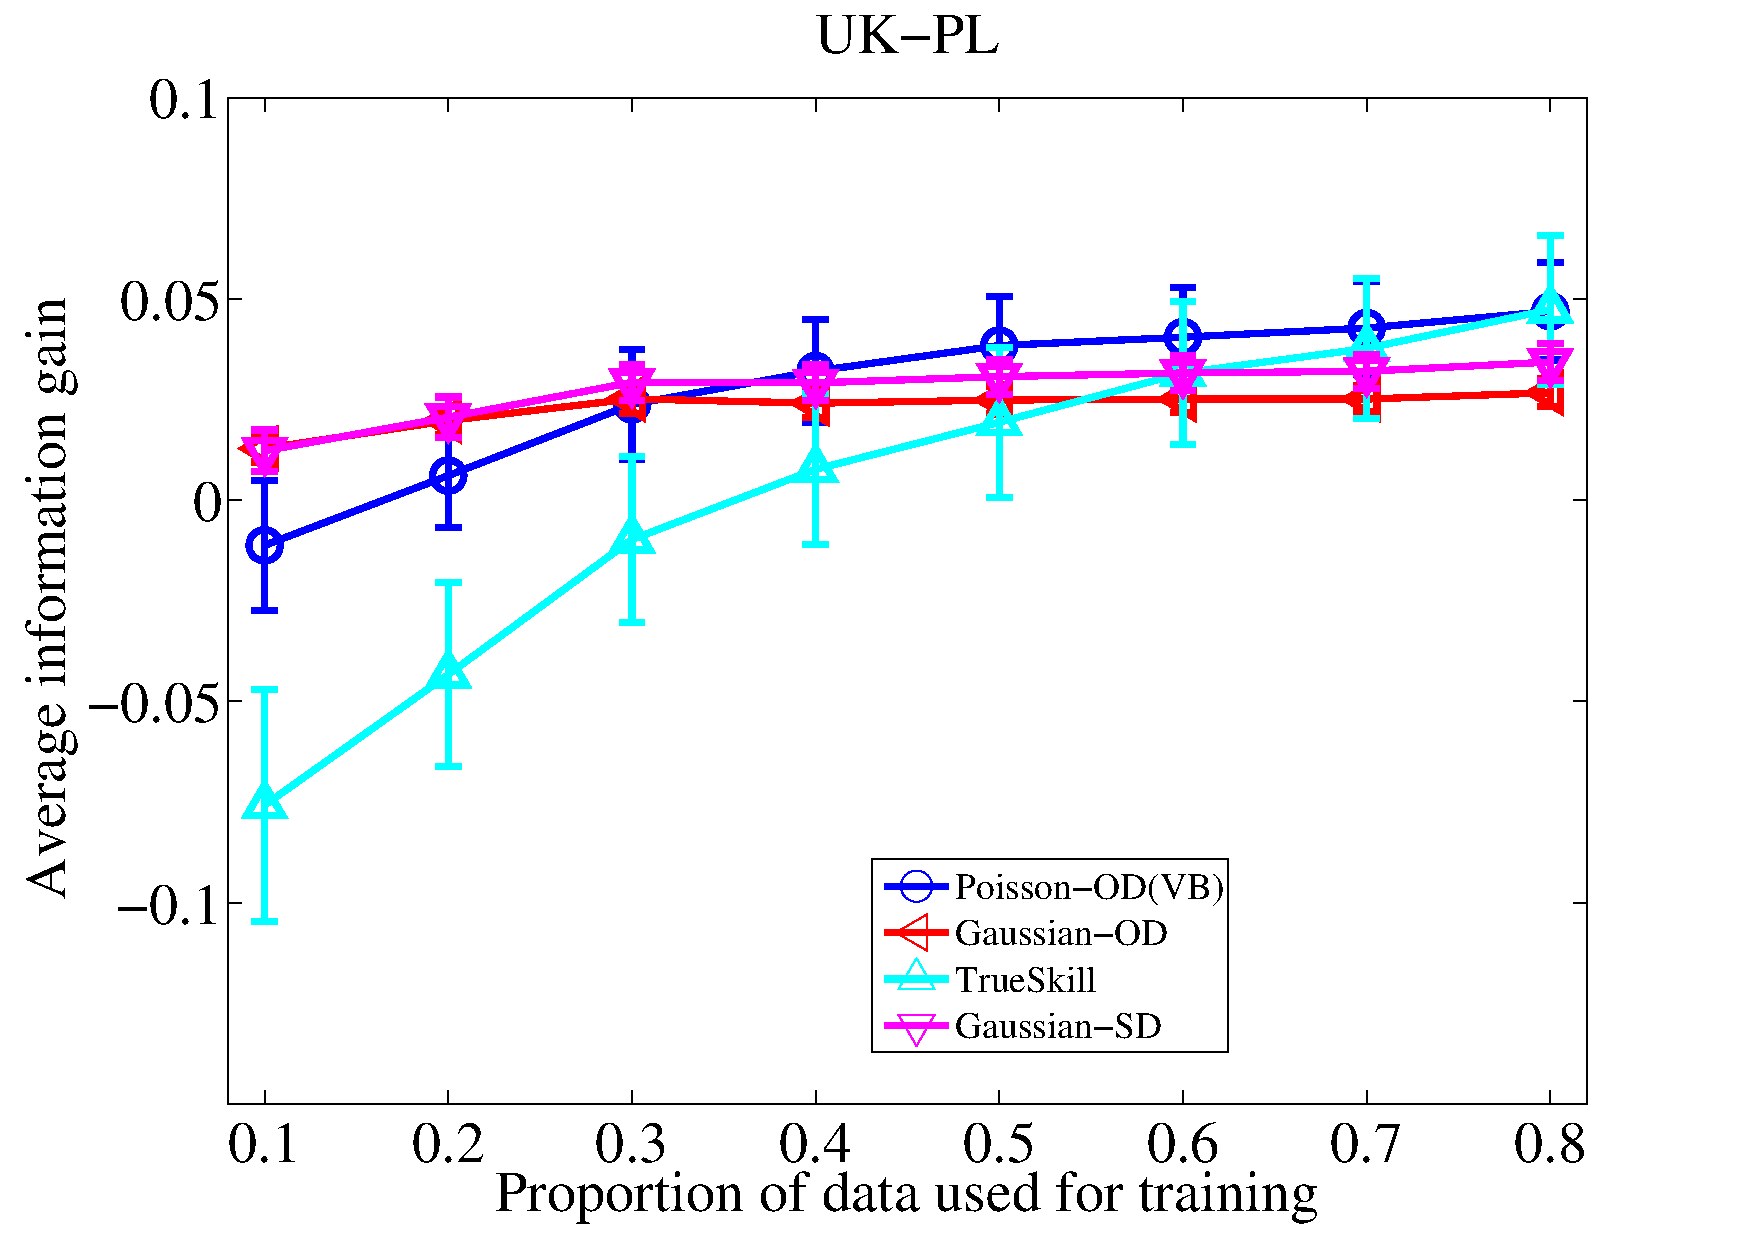
\epsfig{file=InforGain_UK, angle=0, height=7cm} 
}\\
\subfigure{ 
 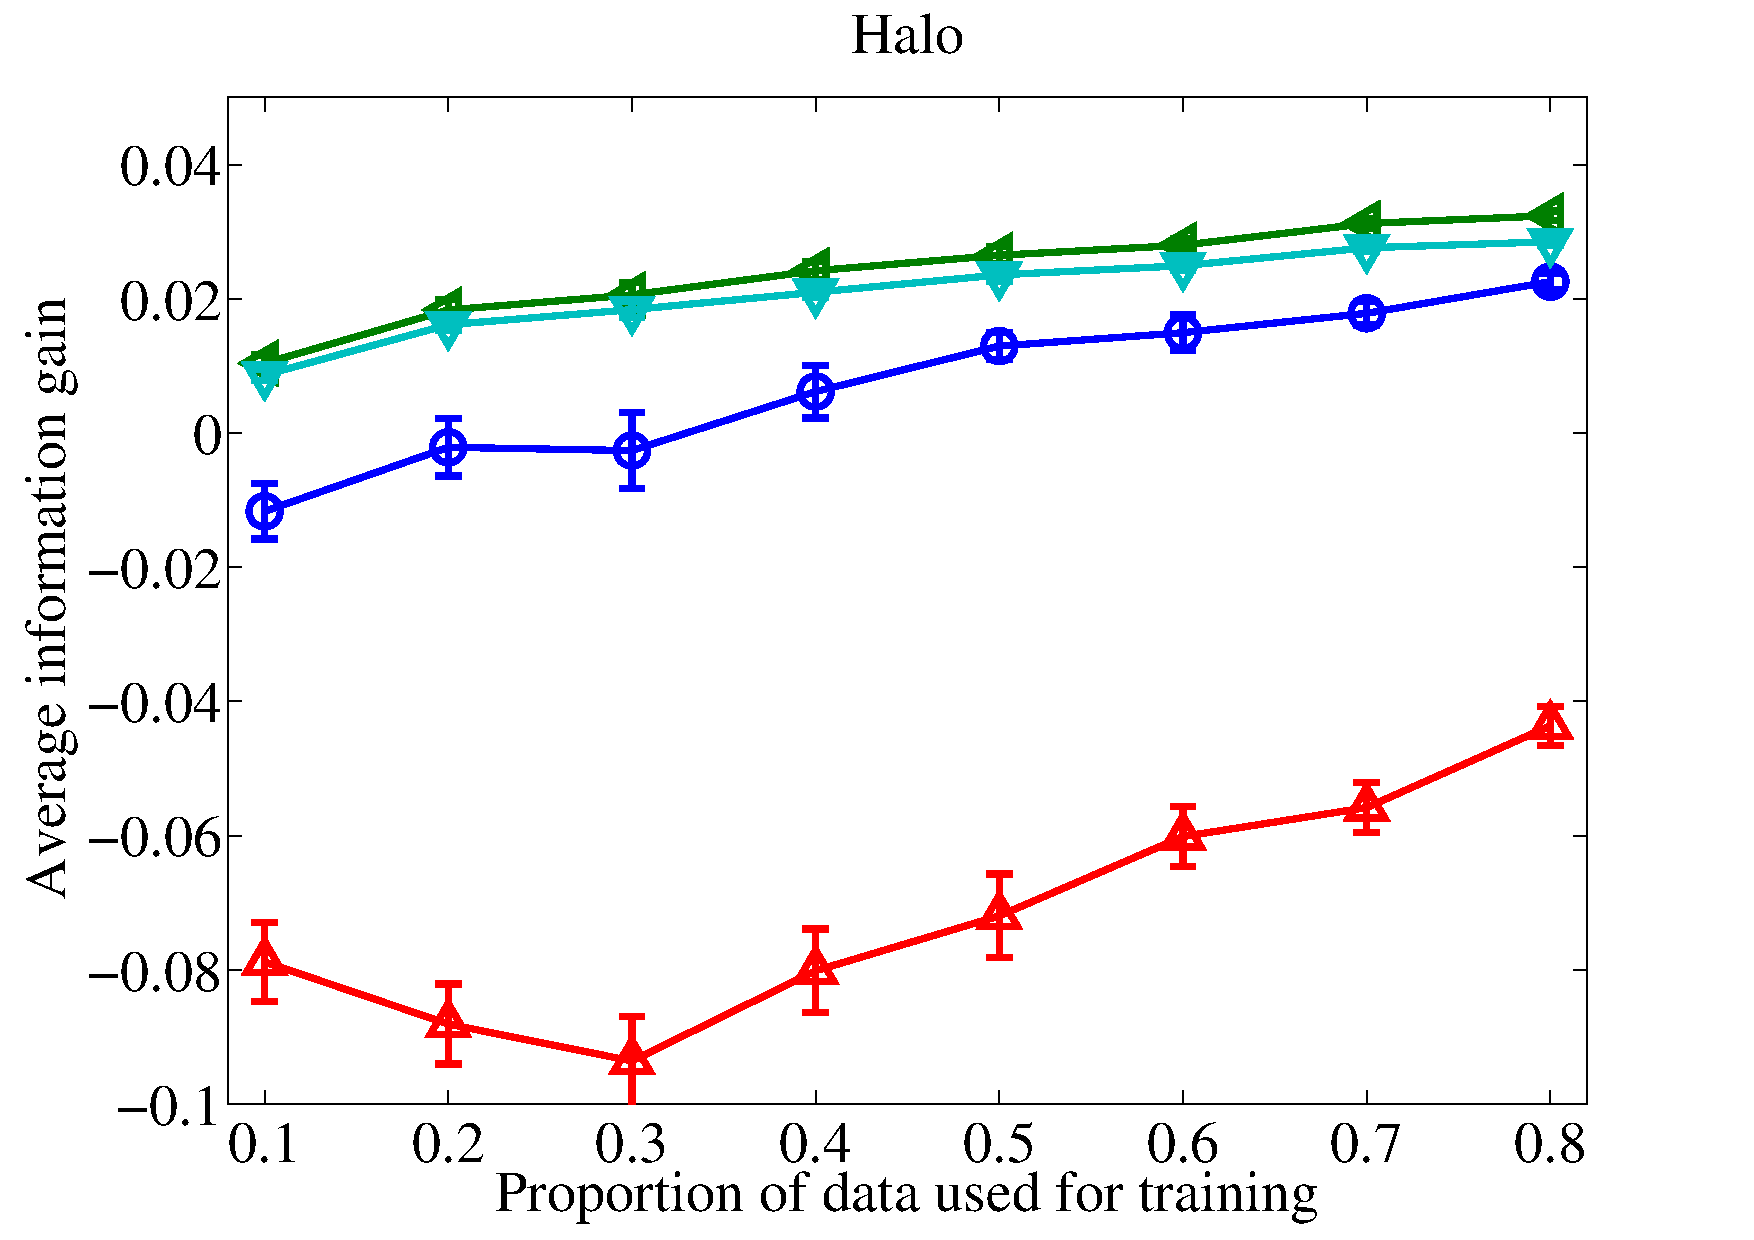
\epsfig{file=InforGain_Halo, angle=0, height=7cm} 
}\\
\subfigure{ 
 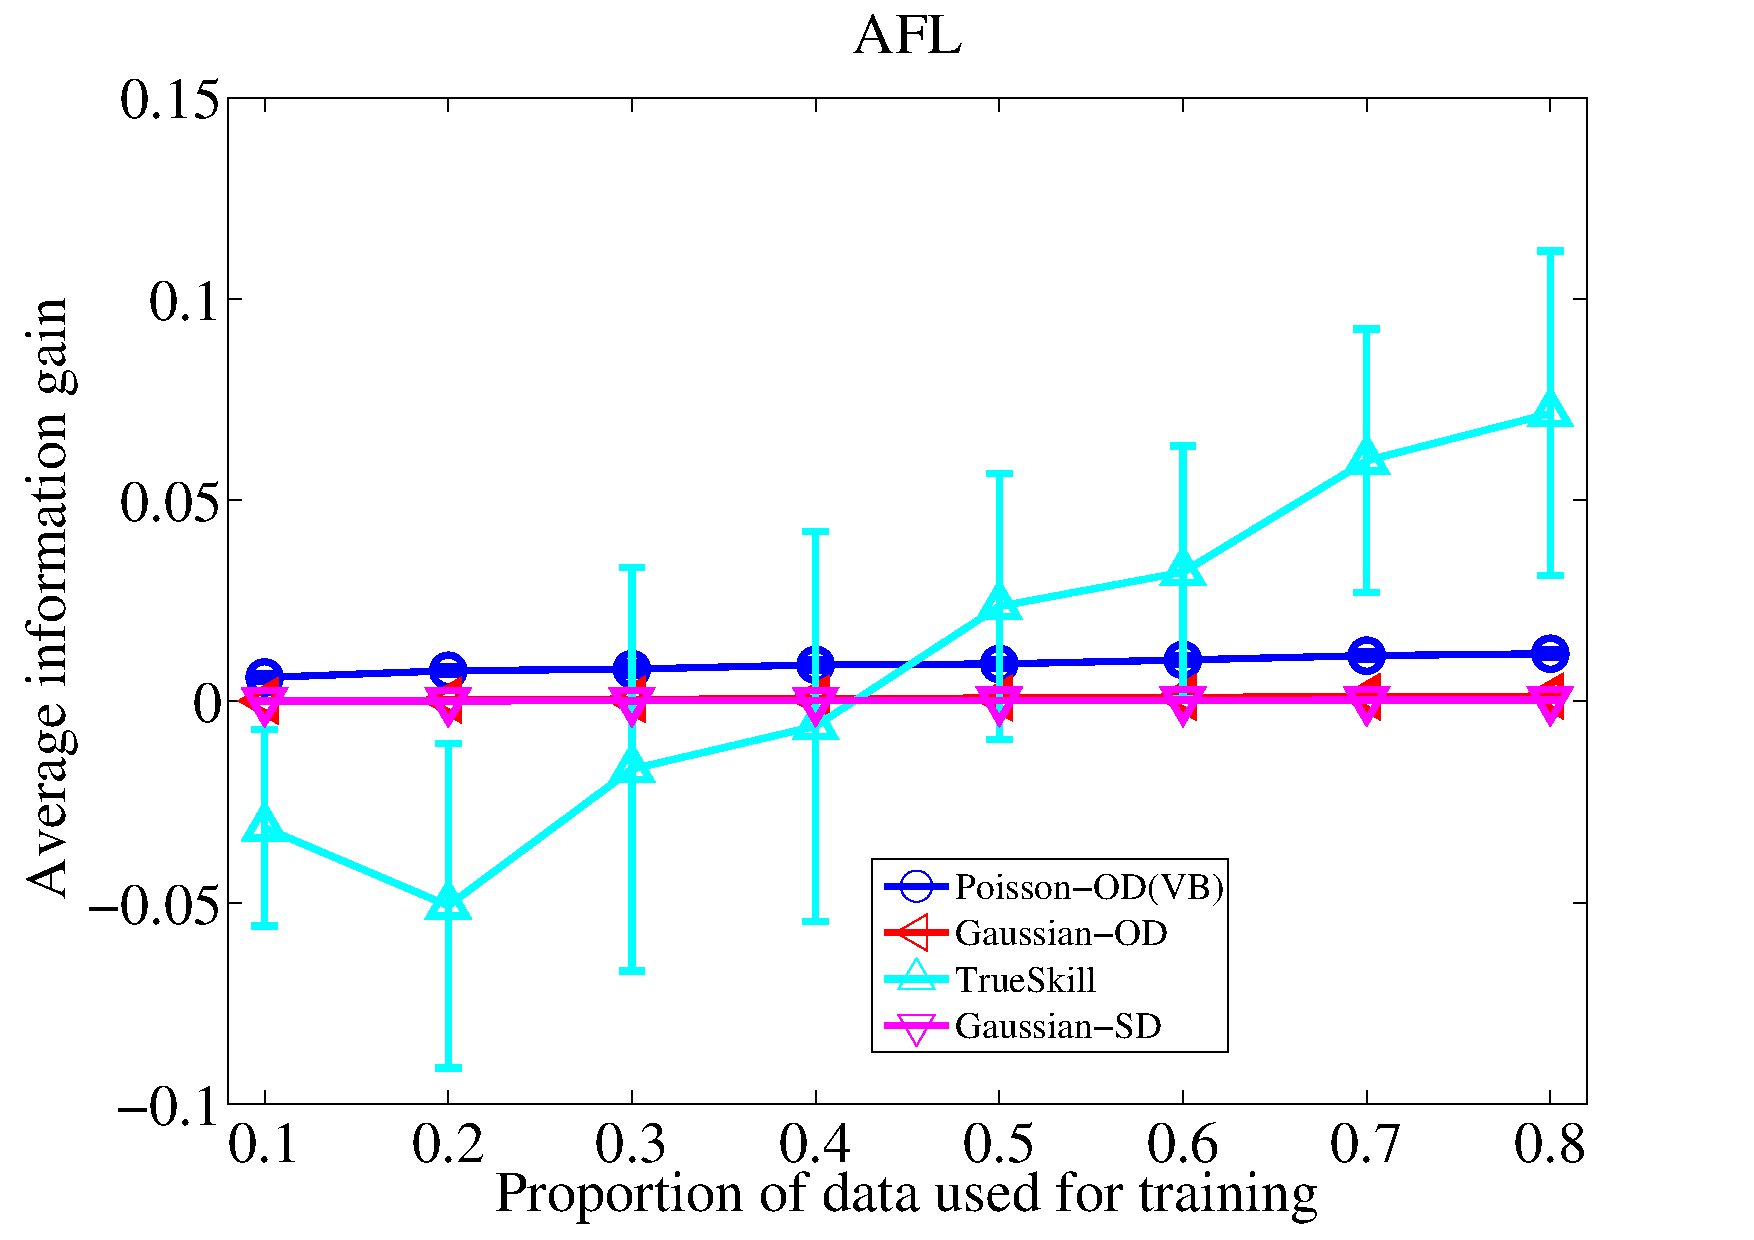
\epsfig{file=InforGain_AFL, angle=0, height=7cm} 
}\\
\caption{\small Results on the UK-PL (upper), Halo (middle), and AFL (bottom), evaluated
using information gain. Error bars indicate
95\% confidence intervals.}
\label{fig:InforGain}
\end{figure}
\end{center}

%\subsubsection{Win/no-Win Prediction Accuracy }
%
%In terms of win/no-win prediction accuracy on the three data sets (Figure~\ref{fig:WLAccuracy}), the Gaussian-OD model generally provides the best average AUC, followed by Gaussian-SD, then
%TrueSkill, then Poisson-OD model. The better performance achieved by the Gaussian-OD model again indicated the benefits of separating offence/defence skill modeling in the Gaussian-OD model, achieving a performance edge over the combined skill model of the Gaussian-SD model.
%
%\begin{center}
%\begin{figure*}[htbp!]
% \centering
% \subfigure{
% 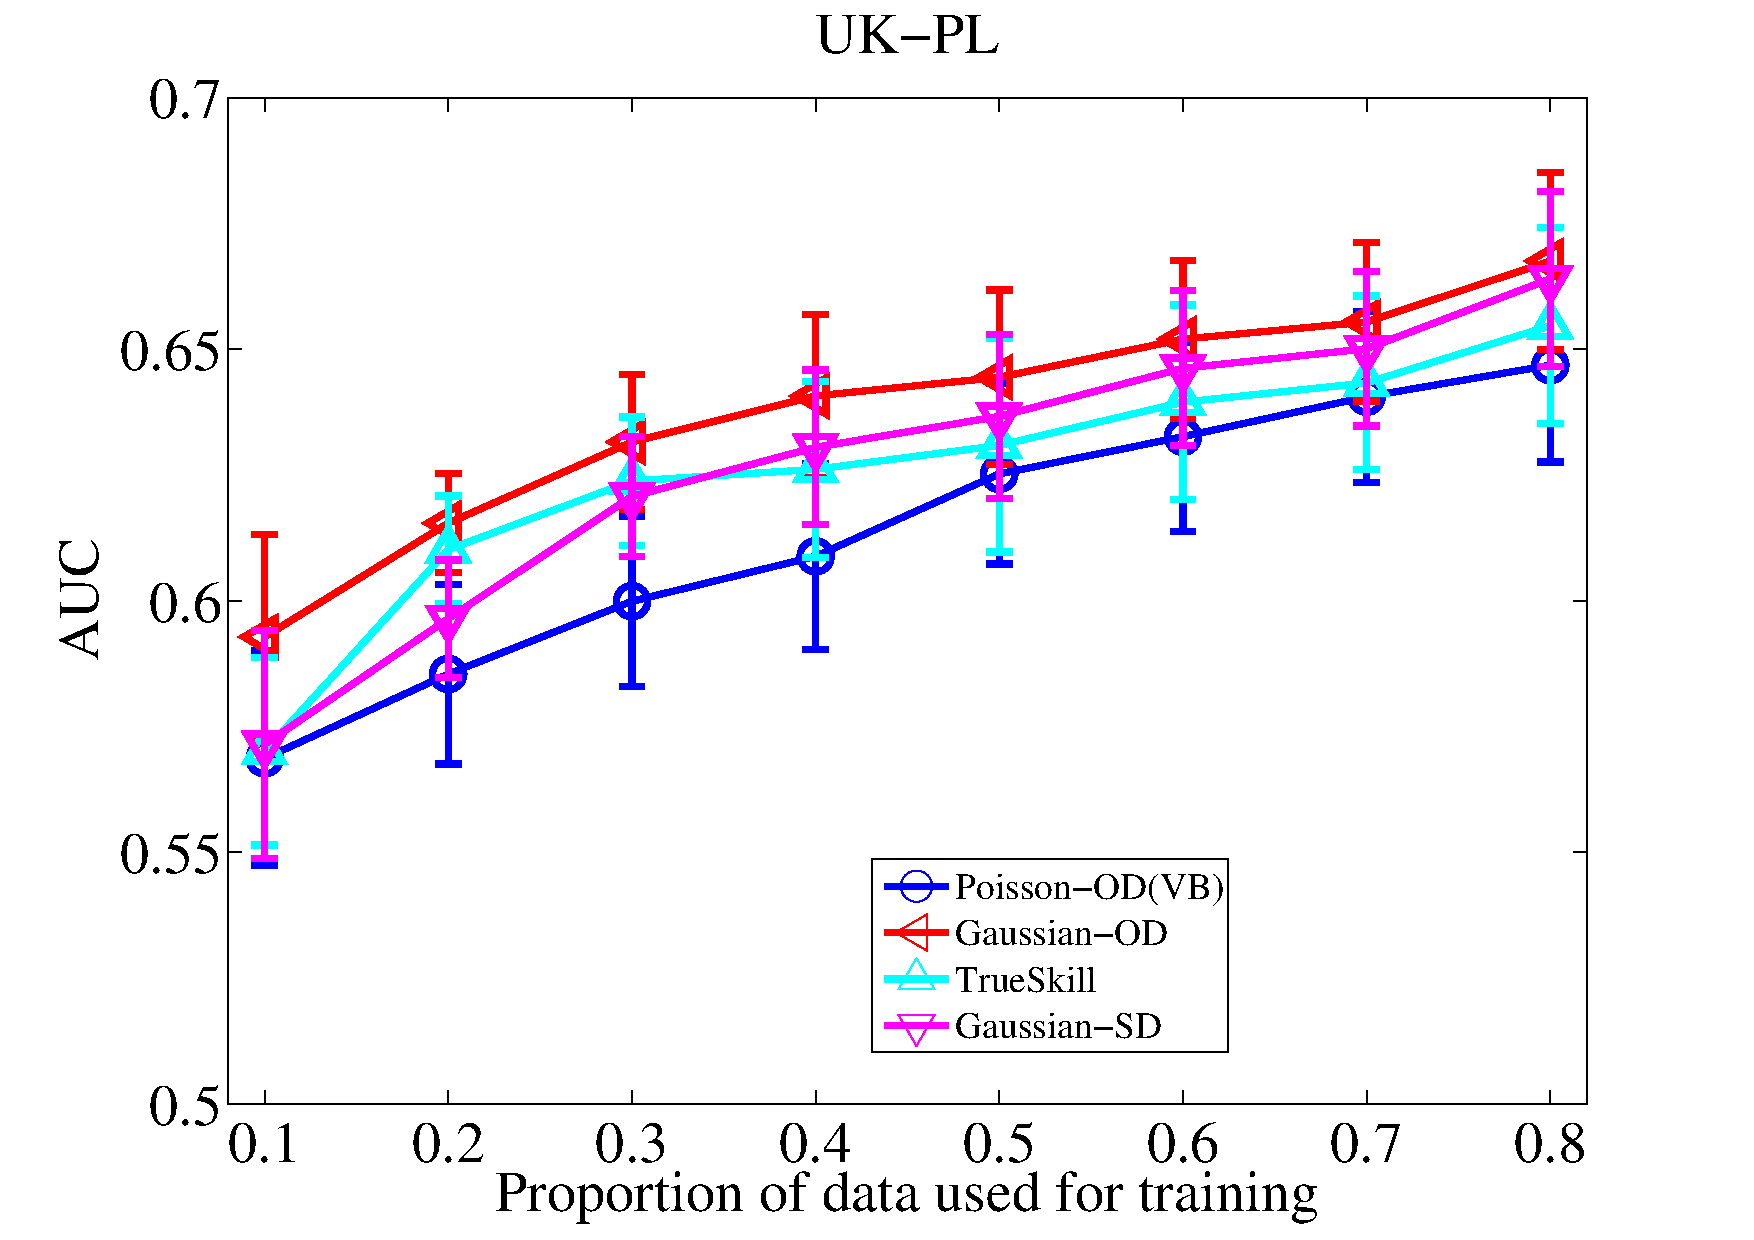
\epsfig{file=WLAccuracy_UK, angle=0, height=8cm} 
%}\\
%\subfigure{ 
% 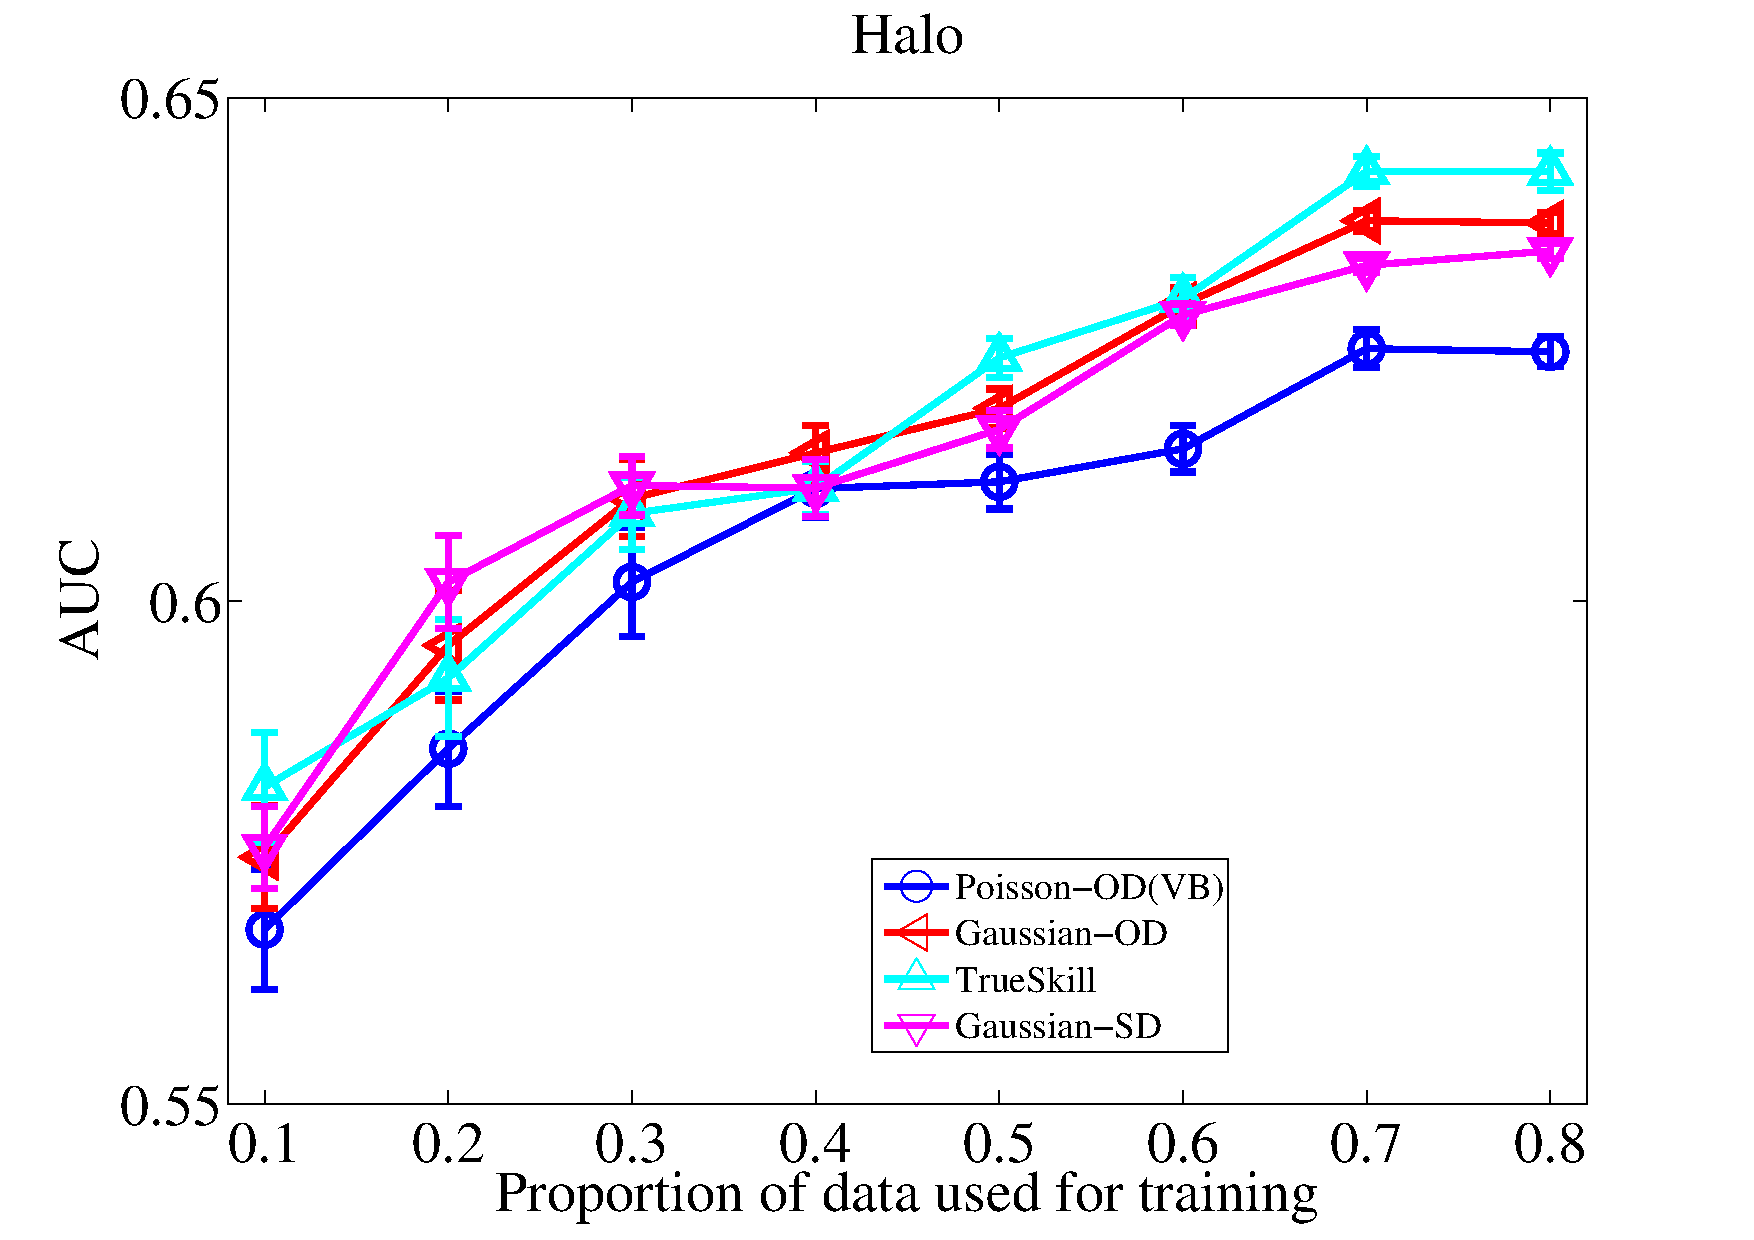
\epsfig{file=WLAccuracy_Halo, angle=0, height=8cm} 
%}\\
%\subfigure{ 
% 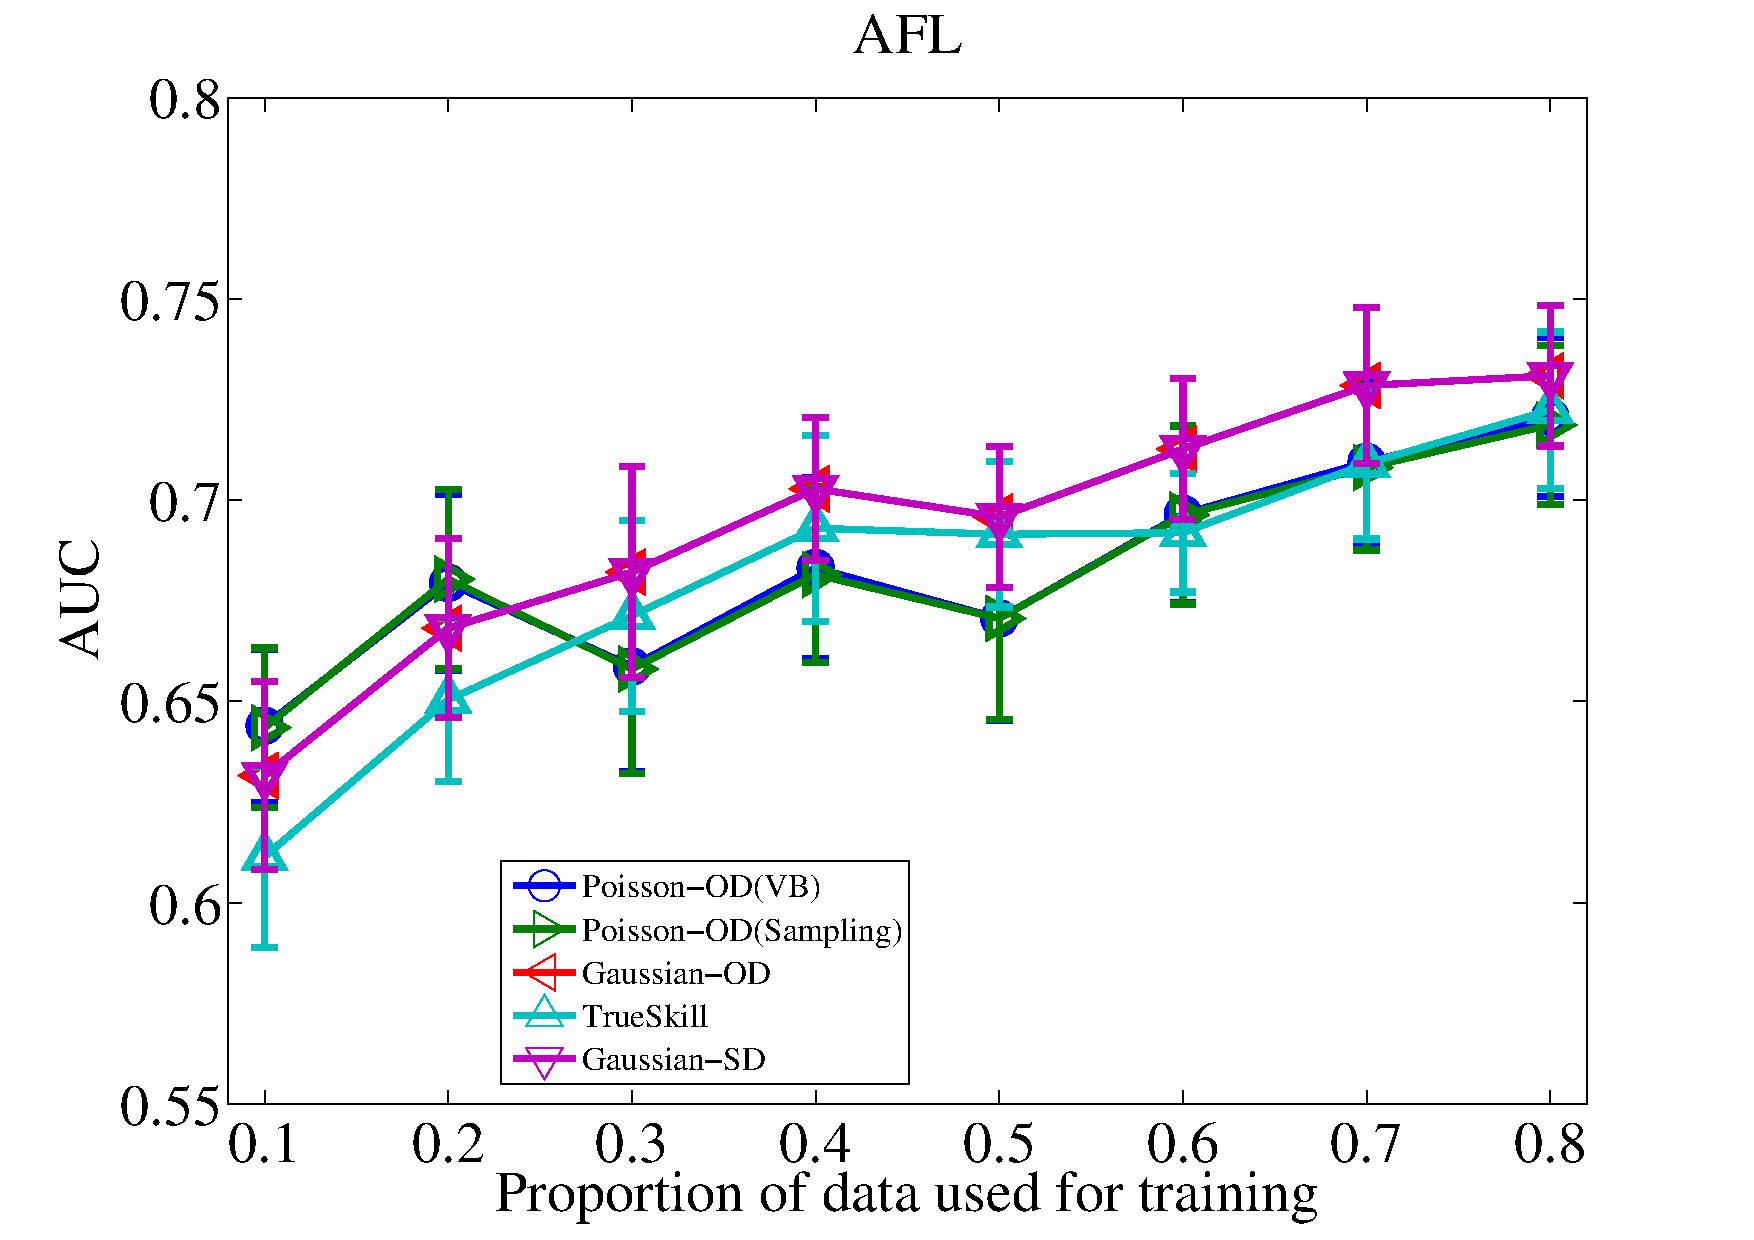
\epsfig{file=WLAccuracy_AFL, angle=0, height=8cm} 
%}\\
%\caption{\small Results on the UK-PL (upper), Halo (middle), and AFL (bottom), evaluated
%using Win/nonWin Accuracy. Error bars indicate
%95\% confidence intervals.}
%\label{fig:WLAccuracy}
%\end{figure*}
%\end{center}

%We check the statistics of the match outcomes
%(Table~\ref{table:datasetStatistics}),
%and observe that the average
%scores for the UK-PL, Halo, and AFL datasets are 1.3, 42.7, and 95.4,
%respectively.  From this, we might infer the Poisson-OD model predicts better
%when the average scores for a dataset are relatively larger numbers;
%here it seems the exponential term used in the Poisson model can help
%amplify small performance differences to explain high scores, leading
%to more stable skill modeling in high-scoring games.

\subsubsection{Win/Lose/Draw Prediction Accuracy}
We further studied the performances of various models under a multi-class classification setting of predicting WLD for a match between two teams $(i, j)$. 
For the results on the UK data set shown in Figure~\ref{fig:accuracyWLD} (Top panel), the best performing model is the Gaussian-OD-AH, which achieved significantly better performance than that for the Gaussian-OD, indicating the importance of introducing the home field advantage variable. Together with the Gaussian-SD model, these three models significantly outperform TrueSkill for all the training settings. For limited training data, the proposed Poisson-OD and Poisson-OD-VB-AH models outperform TrueSkill as well, indicating the importance of modeling scores. 

Results on the Halo data set Figure~\ref{fig:accuracyWLD} (Middle panel) again demonstrated that the proposed models obtained much better WLD predictions comparing with TrueSkill. For this data set, the Gaussian models outperform the Poisson-OD model, which was not surprising as the average score for the Halo data set is relatively small numbers. Note that the performances for the Gaussian models were comparable with each other, which suggested that it may not be beneficial to model offence/defence skills separately for applications where the notions of offence and defence are not clear, which is the case for the Halo data but not for the AFL and UK data sets. 

For the results on the AFL data set in Figure~\ref{fig:accuracyWLD} (Bottom panel),  we observed that the Poisson-OD, Gaussian-SD, Gaussian-OD, and Poisson-OD(VB)-AH all significantly outperformed TrueSkill, which further supported the importance of learning team skills by taking into account the score information. For the Poisson likelihood based models, we observed that when training data was limited, the introduction of the home field advantage variable actually hurt the performance, as shown in Figure~\ref{fig:accuracyWLD} (Bottom panel) when less or equal to 40\% of data was used for training. But with the increasing amount of training data, the refined home advantage variable can help to achieve better performance compared with the Poisson-OD(VB), indicating the marginal benefits of modeling home field advantages. Another observation was that the Possion-OD(VB) achieved the comparable performance with that of the Poisson-OD(Sampling). 

When comparing the best performance across the three data sets for all the models, we note that the mean accuracies for all the models on the AFL data set were the largest than that for the UK data sets, perhaps indicating that football games may be much harder than that the rugby games for AFL. The difficulty in predicting win/lose/draw for football matches is perhaps caused by the unexpected player injuries, teams trading players, etc. One may argue that these factors apply to the AFL data set, but it seems that the AFL has somehow stricter rules in regulating the trading of players. 

\begin{center}
\begin{figure}[htbp!]
 \centering
 \subfigure{
 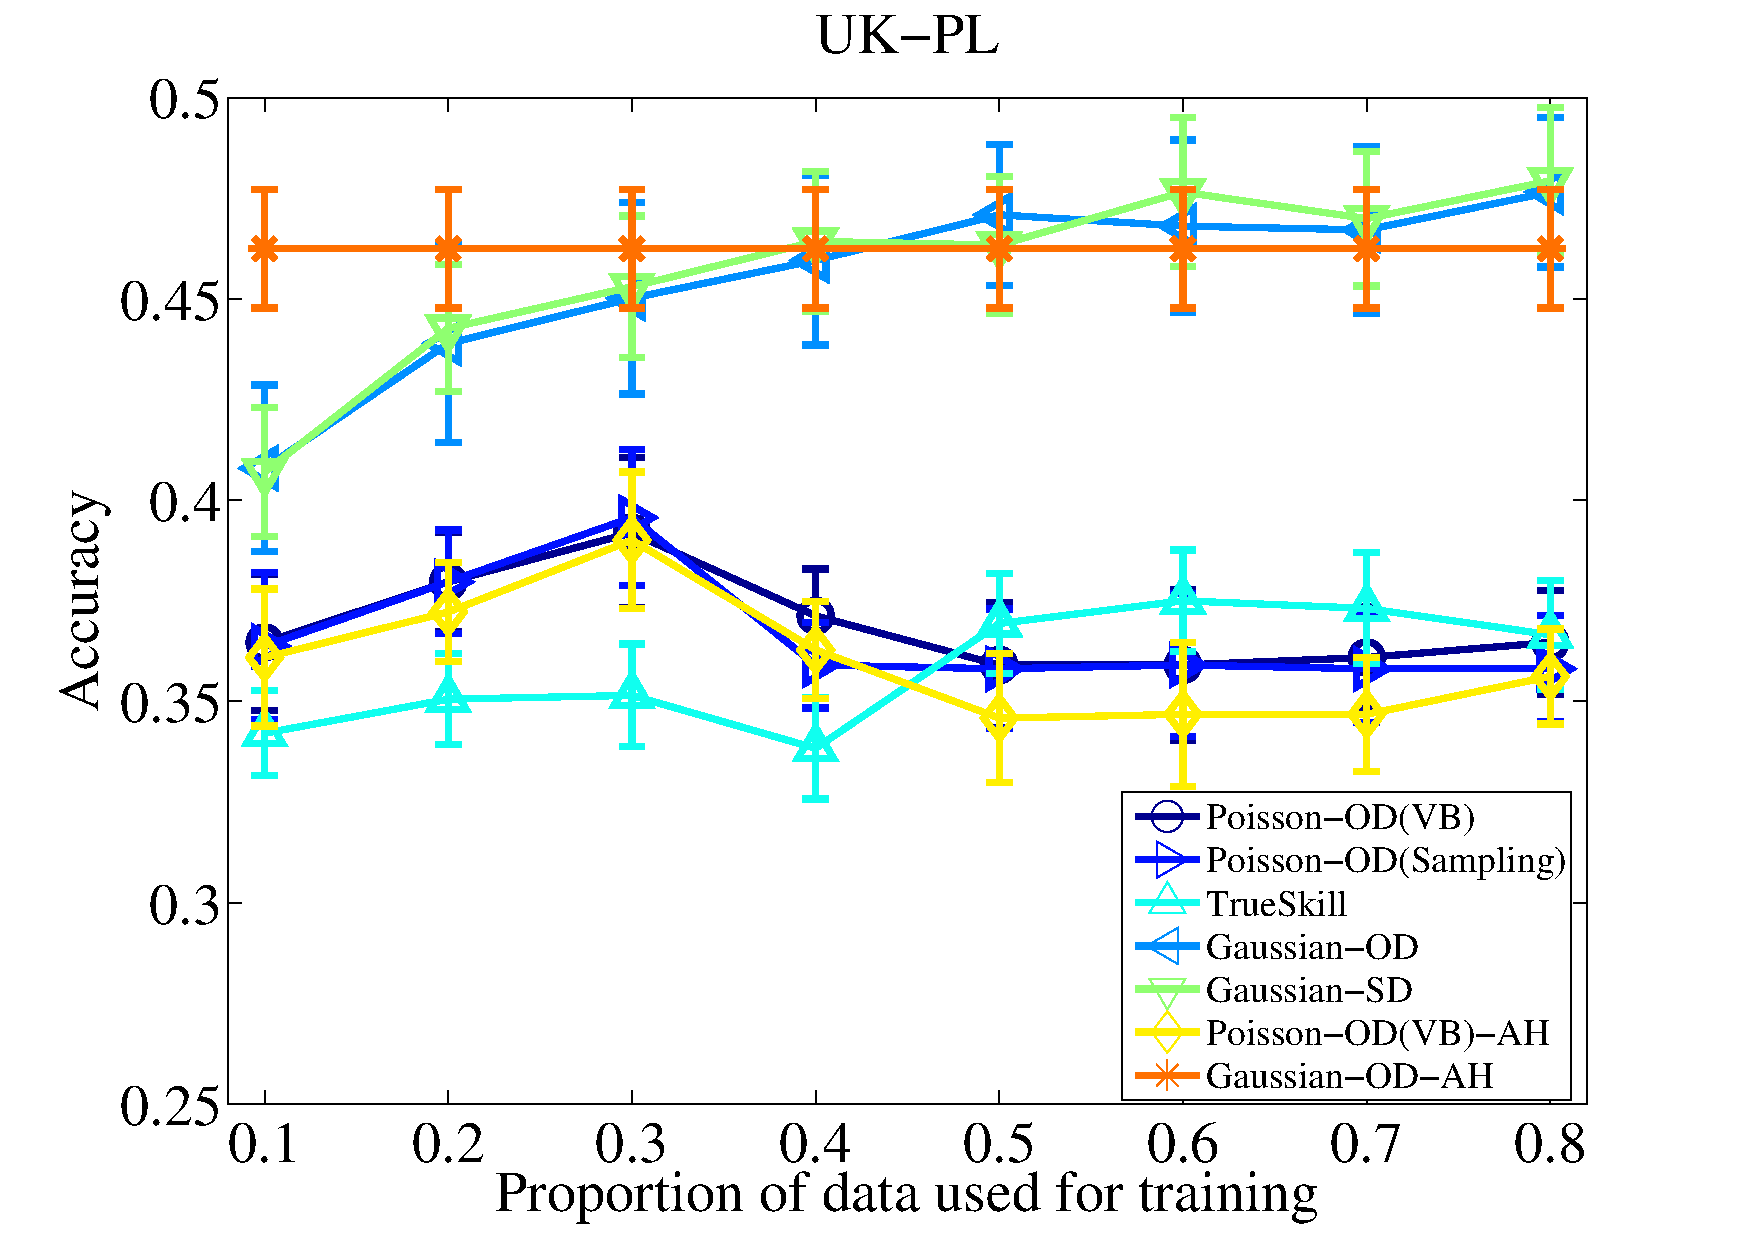
\epsfig{file=accuracy_UK, angle=0, height=7cm} 
}\\
\subfigure{ 
 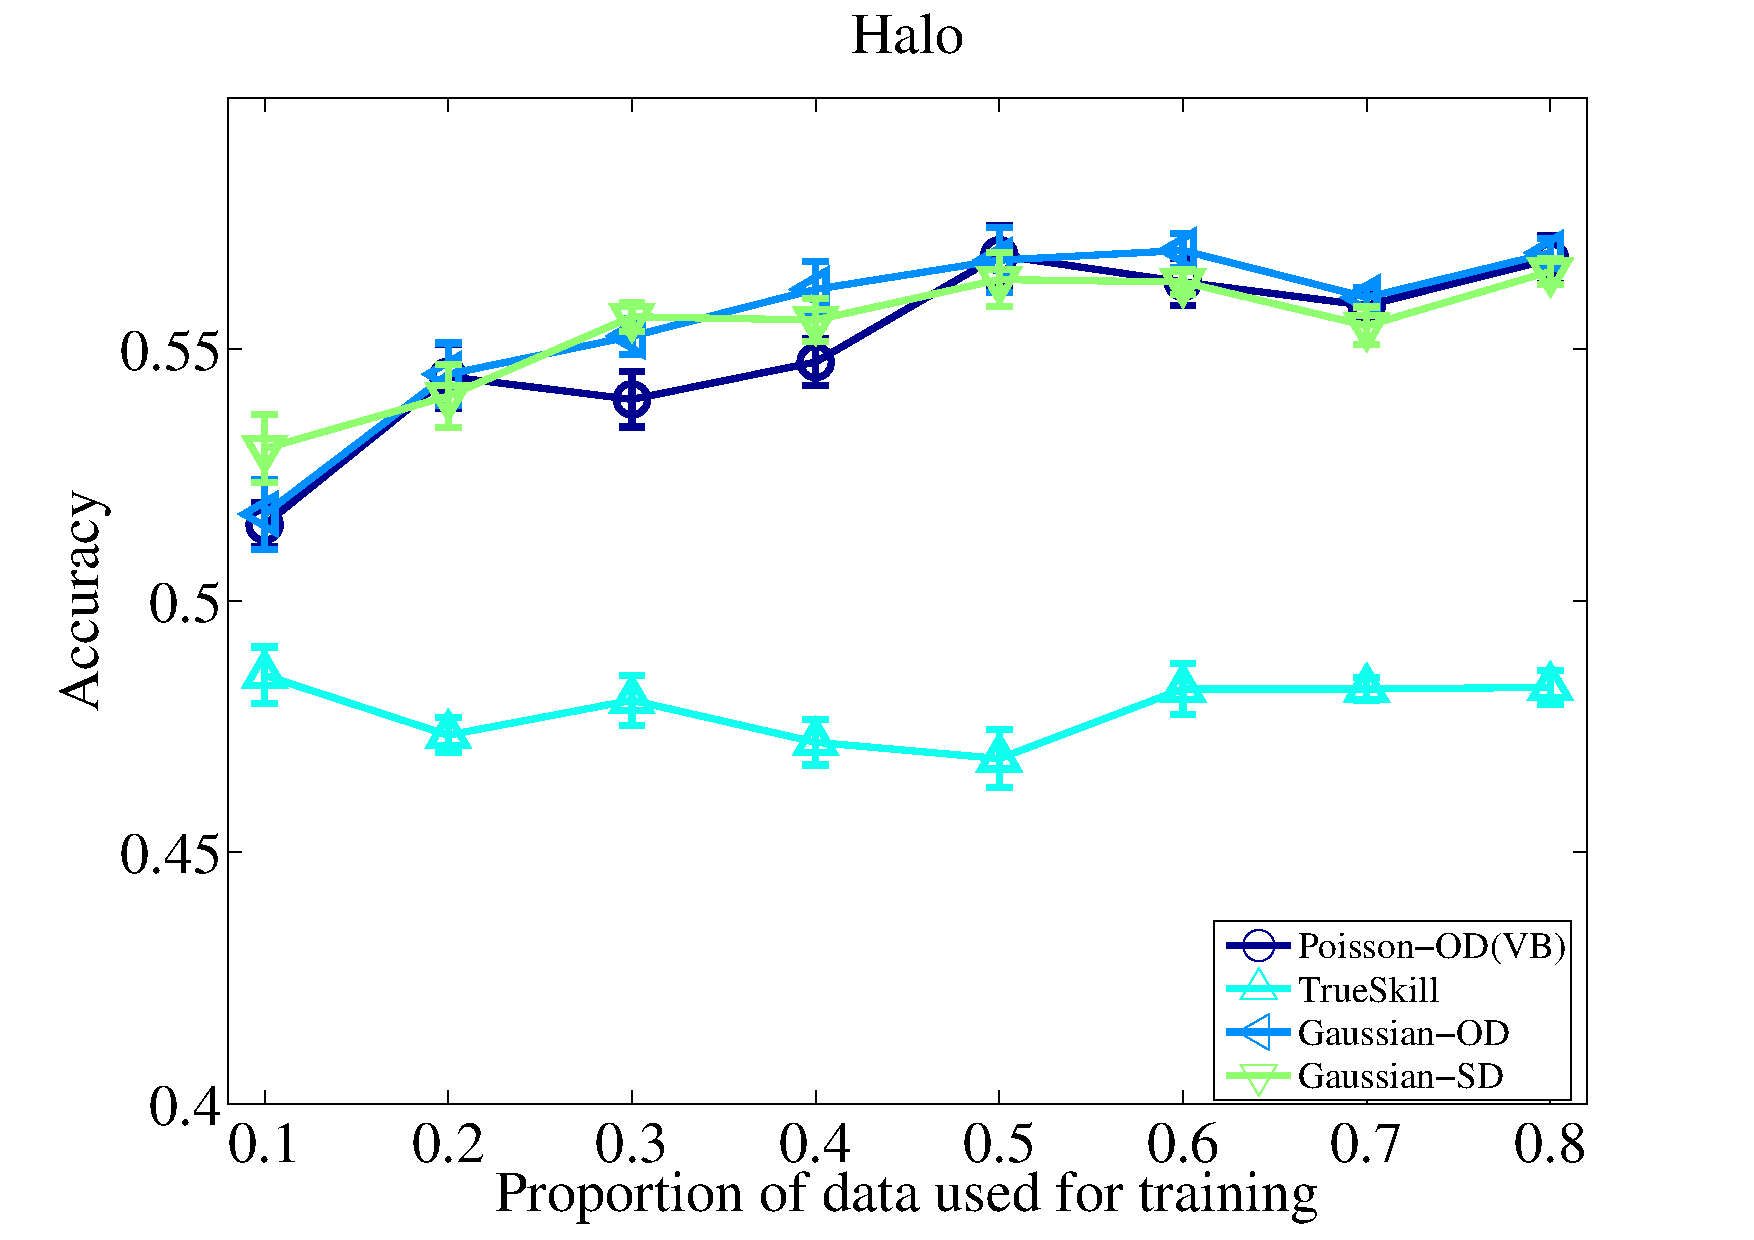
\epsfig{file=accuracy_Halo, angle=0, height=7cm} 
}\\
\subfigure{ 
 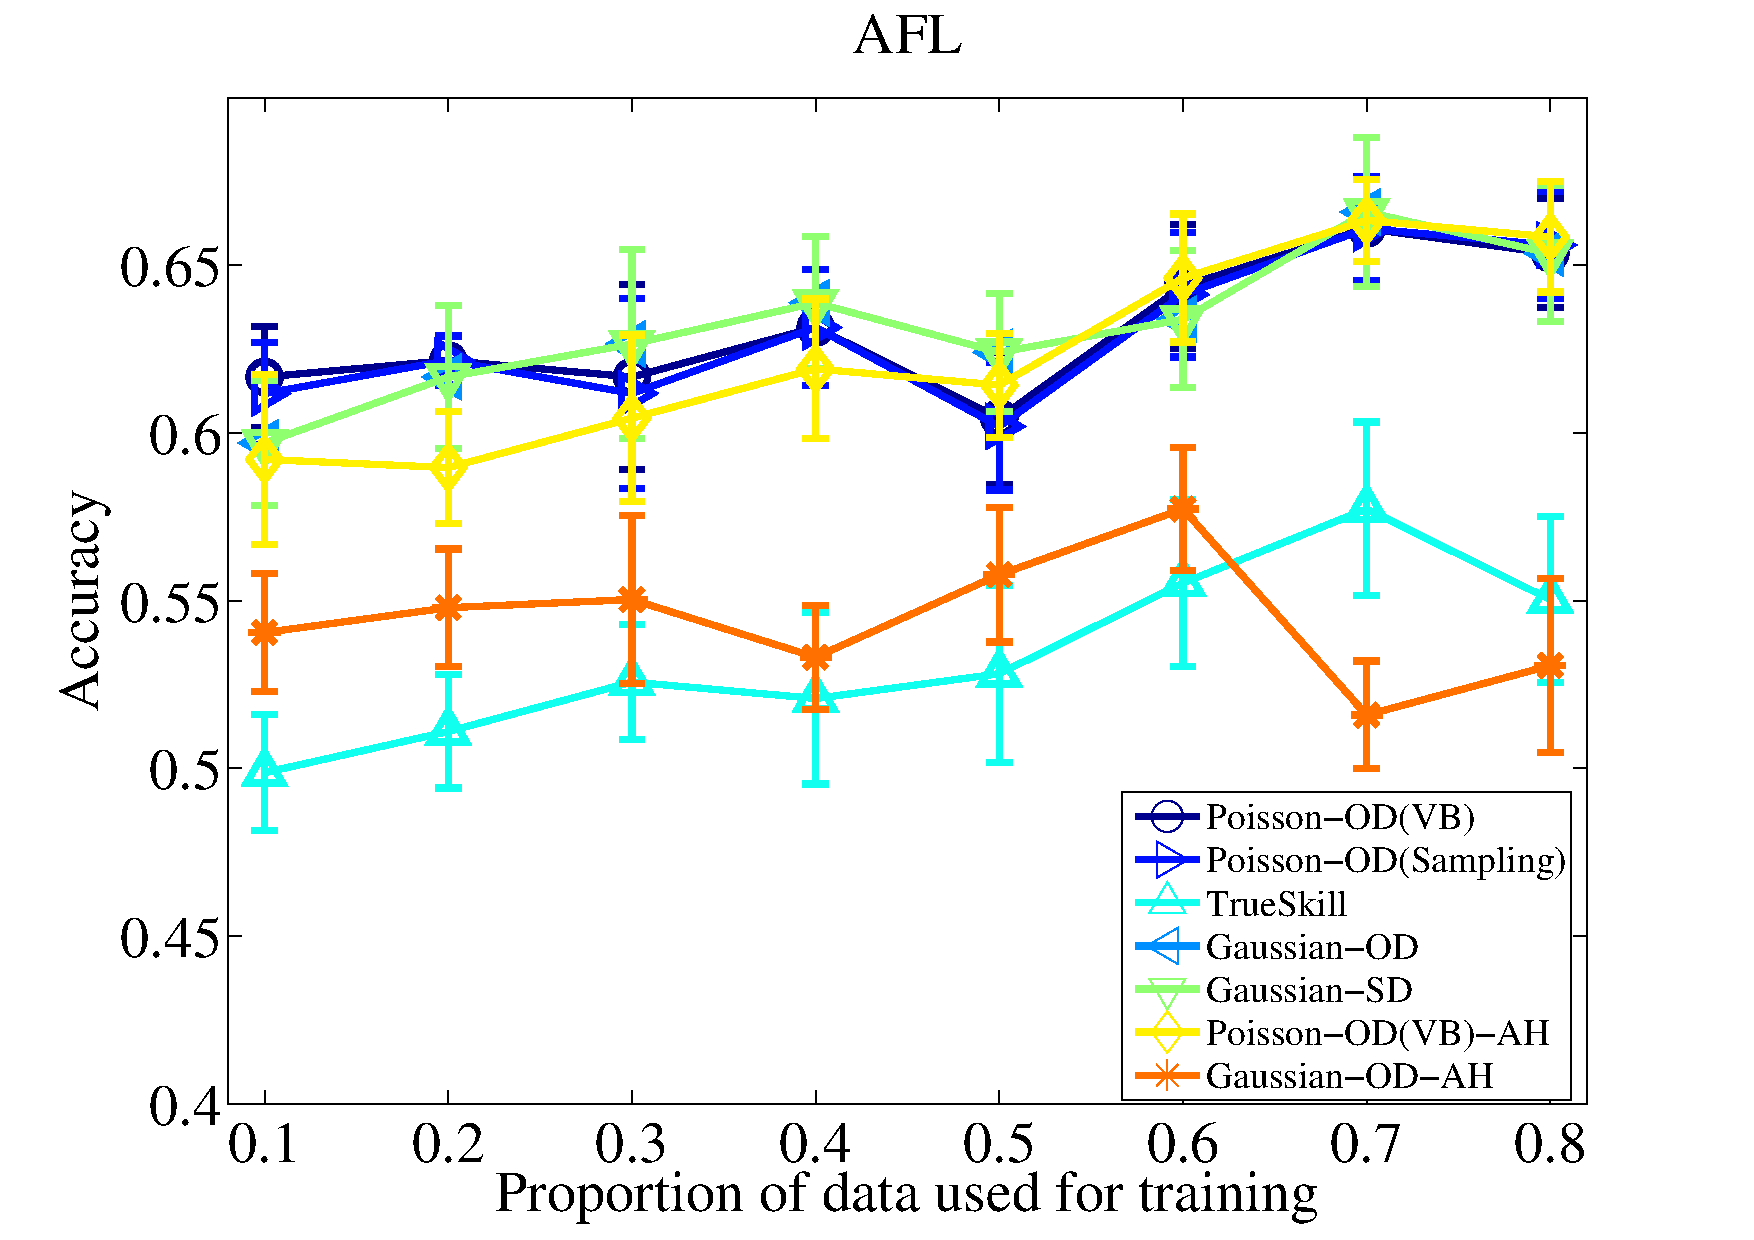
\epsfig{file=accuracy_AFL, angle=0, height=7cm} 
}\\
\caption{\small Results on the UK-PL (Top), Halo (Middle), and AFL (Bottom), evaluated
using the classification accuracy. Error bars indicate
95\% confidence intervals.}
\label{fig:accuracyWLD}
\end{figure}
\end{center}

\subsubsection{Log likelihood}
For the log likelihood on UK data set (Figure~\ref{fig:logLik} Top Panel), we observed that the TrueSkill performed the best across all models for limited data, however, the Poisson models edge out all other models when more than 30\% of data was used for training. For the Gaussian models, the Gaussian-OD and Gaussian-SD models performed comparably with each other. 

For the log-likelihood of the Halo data set show in Figure~\ref{fig:logLik} (Middle Panel), we observed that the Poisson-OD(VB), Gaussian-OD, and Gaussian-SD, outperformed the TrueSkill. Another observation was that the Gaussian-SD model significantly outperformed the Gaussian-OD model, which was not surprising because there were no explicit connections with a player's offence and defence skills for the Halo data set, contrasted with that for the AFL and UK data sets. 

Results on the AFL data set was shown in Figure~\ref{fig:logLik} (Bottom Panel). We observed that the Gaussian-OD-AH, Gaussian-SD, and Gaussian-OD models were the best performing ones comparing with the rest. Amongst these three models, they were comparable with each other. For the Poisson-OD(VB)-AH, it initially performed worse than the Poisson-OD(VB) model, but obtained slightly better performance when more data was used for training. Finally, we observed that there was no distinctions between the Poisson-OD(VB) and Poisson-OD(Sampling). 

\begin{center}
\begin{figure}[htbp!]
 \centering
 \subfigure{
 \epsfig{file=Loglik_UK, angle=0, height=7cm} 
}\\
\subfigure{ 
 \epsfig{file=Loglik_Halo, angle=0, height=7cm} 
}\\
\subfigure{ 
 \epsfig{file=Loglik_AFL, angle=0, height=7cm} 
}\\
\caption{\small Results on the UK-PL (upper), Halo (middle), and AFL (bottom), evaluated
using log likelihood. Error bars indicate
95\% confidence intervals.}
\label{fig:logLik}
\end{figure}
\end{center}

\subsubsection{Score Prediction Errors}
We reported the score prediction errors for different data sets in Figure~\ref{fig:ScoreError}. For the UK data set (Figure~\ref{fig:ScoreError} Top Panel), the Poisson-OD(VB) and Poisson-OD(VB)-AH model clearly did not work well in predicting this type of matches, which are characterized by low match scores (average scores being 1.3 for the UK data set). But the Gaussian-OD and Gaussian-OD-AH models significantly outperformed the baseline for most of the training settings. 

For the results on the Halo dataset (Figure~\ref{fig:ScoreError} Middle Panel), we observed that the proposed Poisson-OD and Gaussian-OD models significantly outperformed the baseline. This demonstrated that our proposed model can make sensible score predictions for online games as well. When comparing between the Poisson-OD and Gaussian models, it is clear that the Gaussian-OD model achieves much better performance.

For the AFL data set in Figure~\ref{fig:ScoreError} (Bottom Panel), we observed that the Gaussian-OD and Gaussian-OD-AH model clearly failed in predicting the scores of the matches, because the differences in the learned skill levels between teams are relatively small. Thus, a Gaussian likelihood function with the small difference has low probability of generating huge match scores for the AFL data set. Given the same difference, the Poisson-OD and Poisson-OD-AH models with an exponentiated scoring rate would seem to amplify these small performance differences in learned AFL skills to make more accurate score predictions on AFL data comparing with the baseline. This amplification appears to hurt the Poisson-OD model on the lower-scoring UK-PL (the mean score for the AFL data is 95.4 vs 42.7 and 1.3 respectively for the Halo 2 and UK-PL data) as shown in Figure~\ref{fig:ScoreError} (Top Panel). Finally, we note that the Poisson-OD(VB) and the Poisson-OD(Sampling) performed comparably with each other. 

We want to emphasize that for the AFL data set, we observe that the baseline method based on average scores of each team makes better predictions than the Poisson model for the single training setting where 10\% of data was used for training. This was not surprising because the belief associated with the Poisson-OD(VB), Poisson-OD(VB)-AH, and Poisson-OD(Sampling) model on team skills exhibited large uncertainty when only a few observations were used for training. As we can see when more data was used for training, all of the Poisson likelihood based models performed significantly better than the baseline. 

\begin{center}
\begin{figure}[htbp!]
 \centering
 \subfigure{
 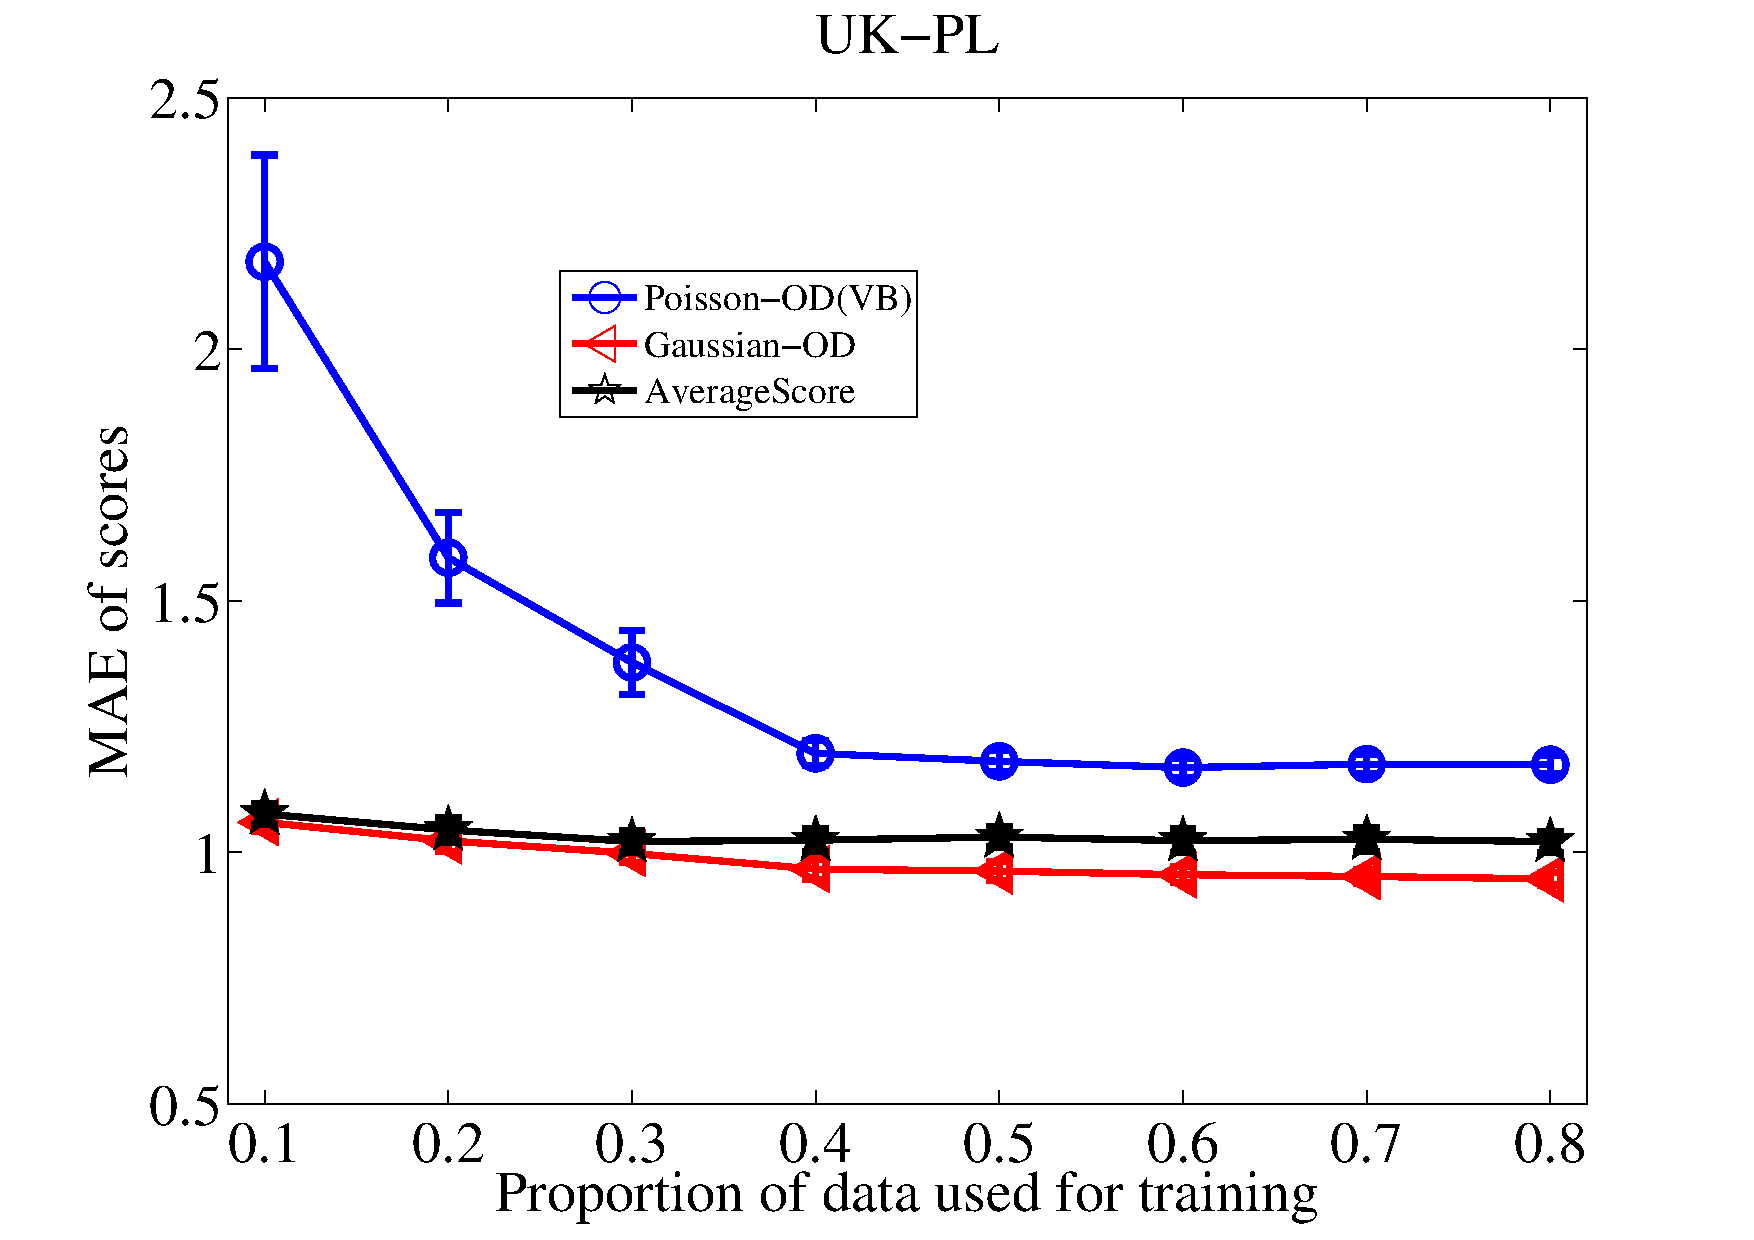
\epsfig{file=ScoreError_UK, angle=0, height=7cm} 
}\\
\subfigure{ 
 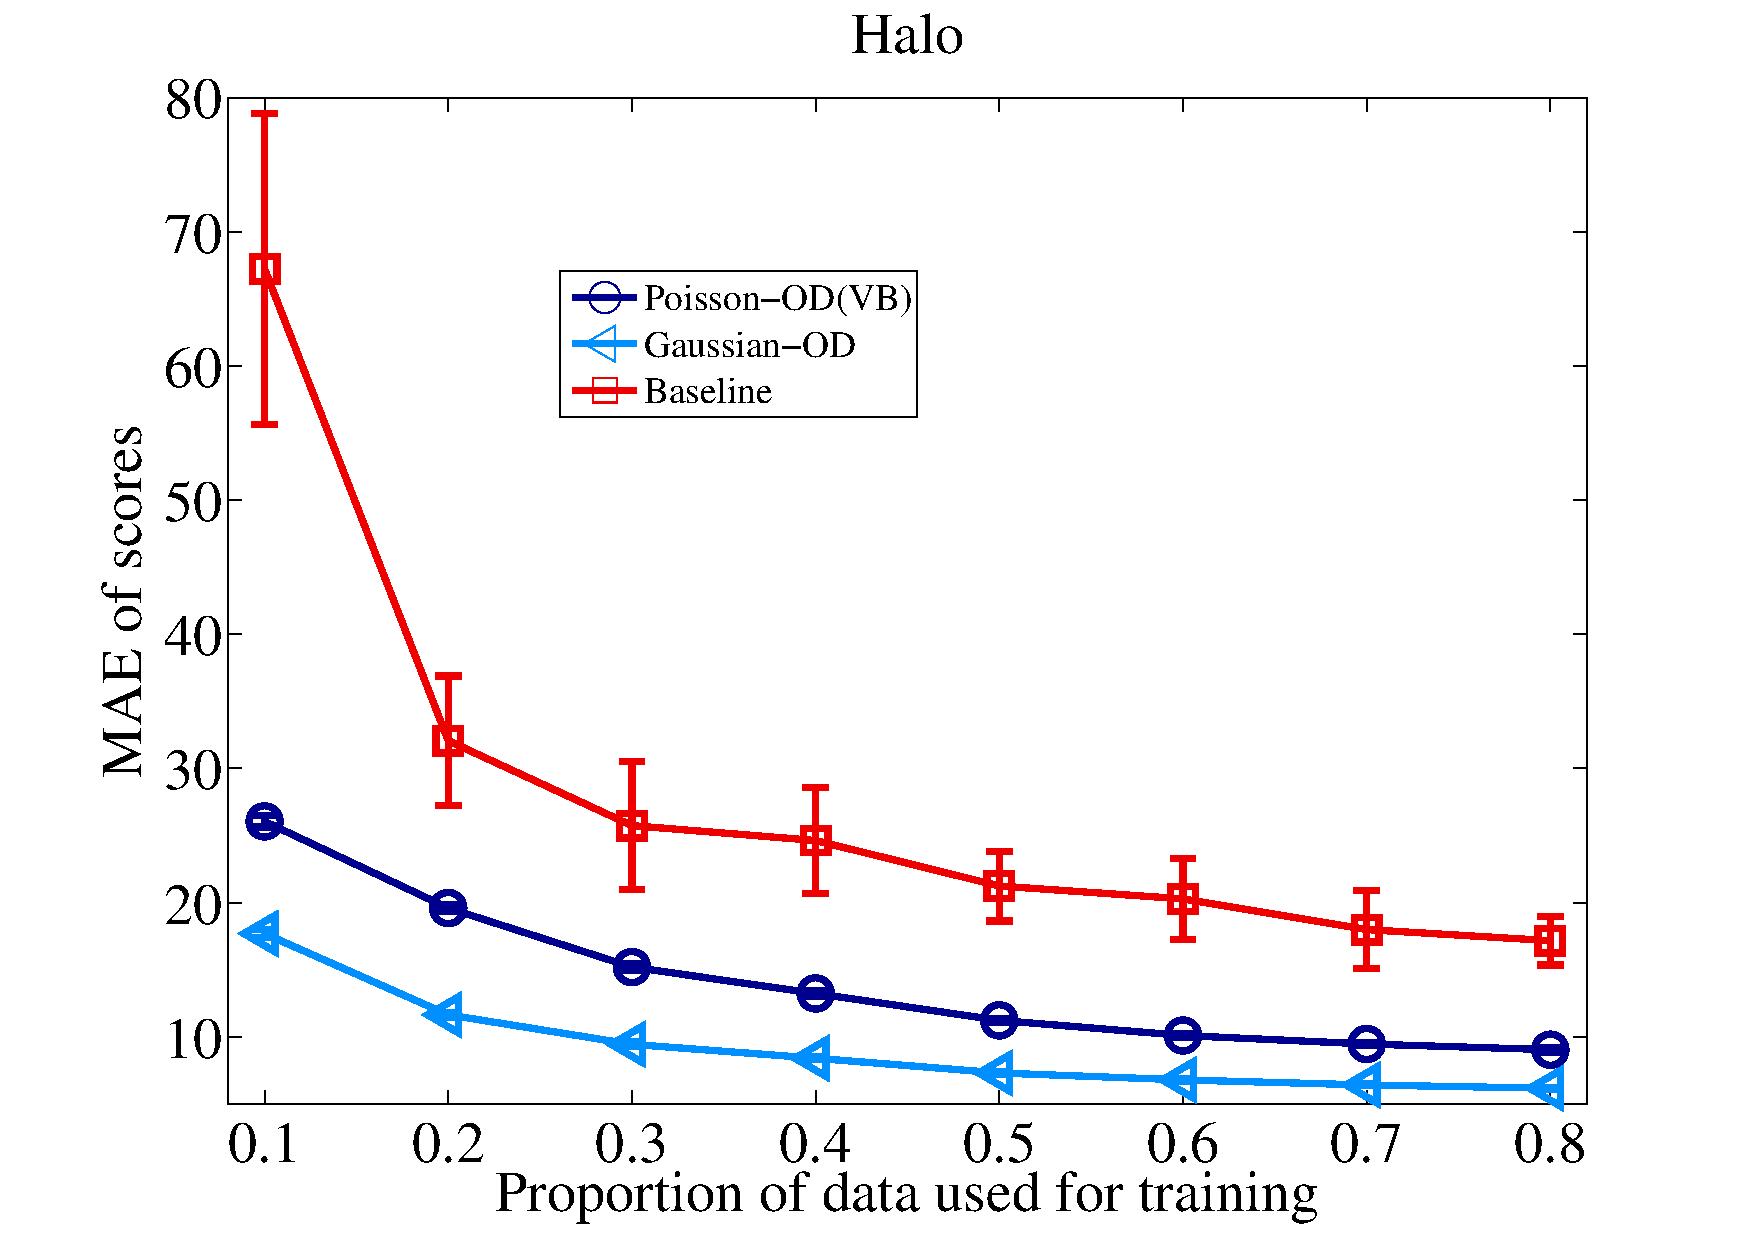
\epsfig{file=ScoreError_Halo, angle=0, height=7cm} 
}\\
\subfigure{ 
 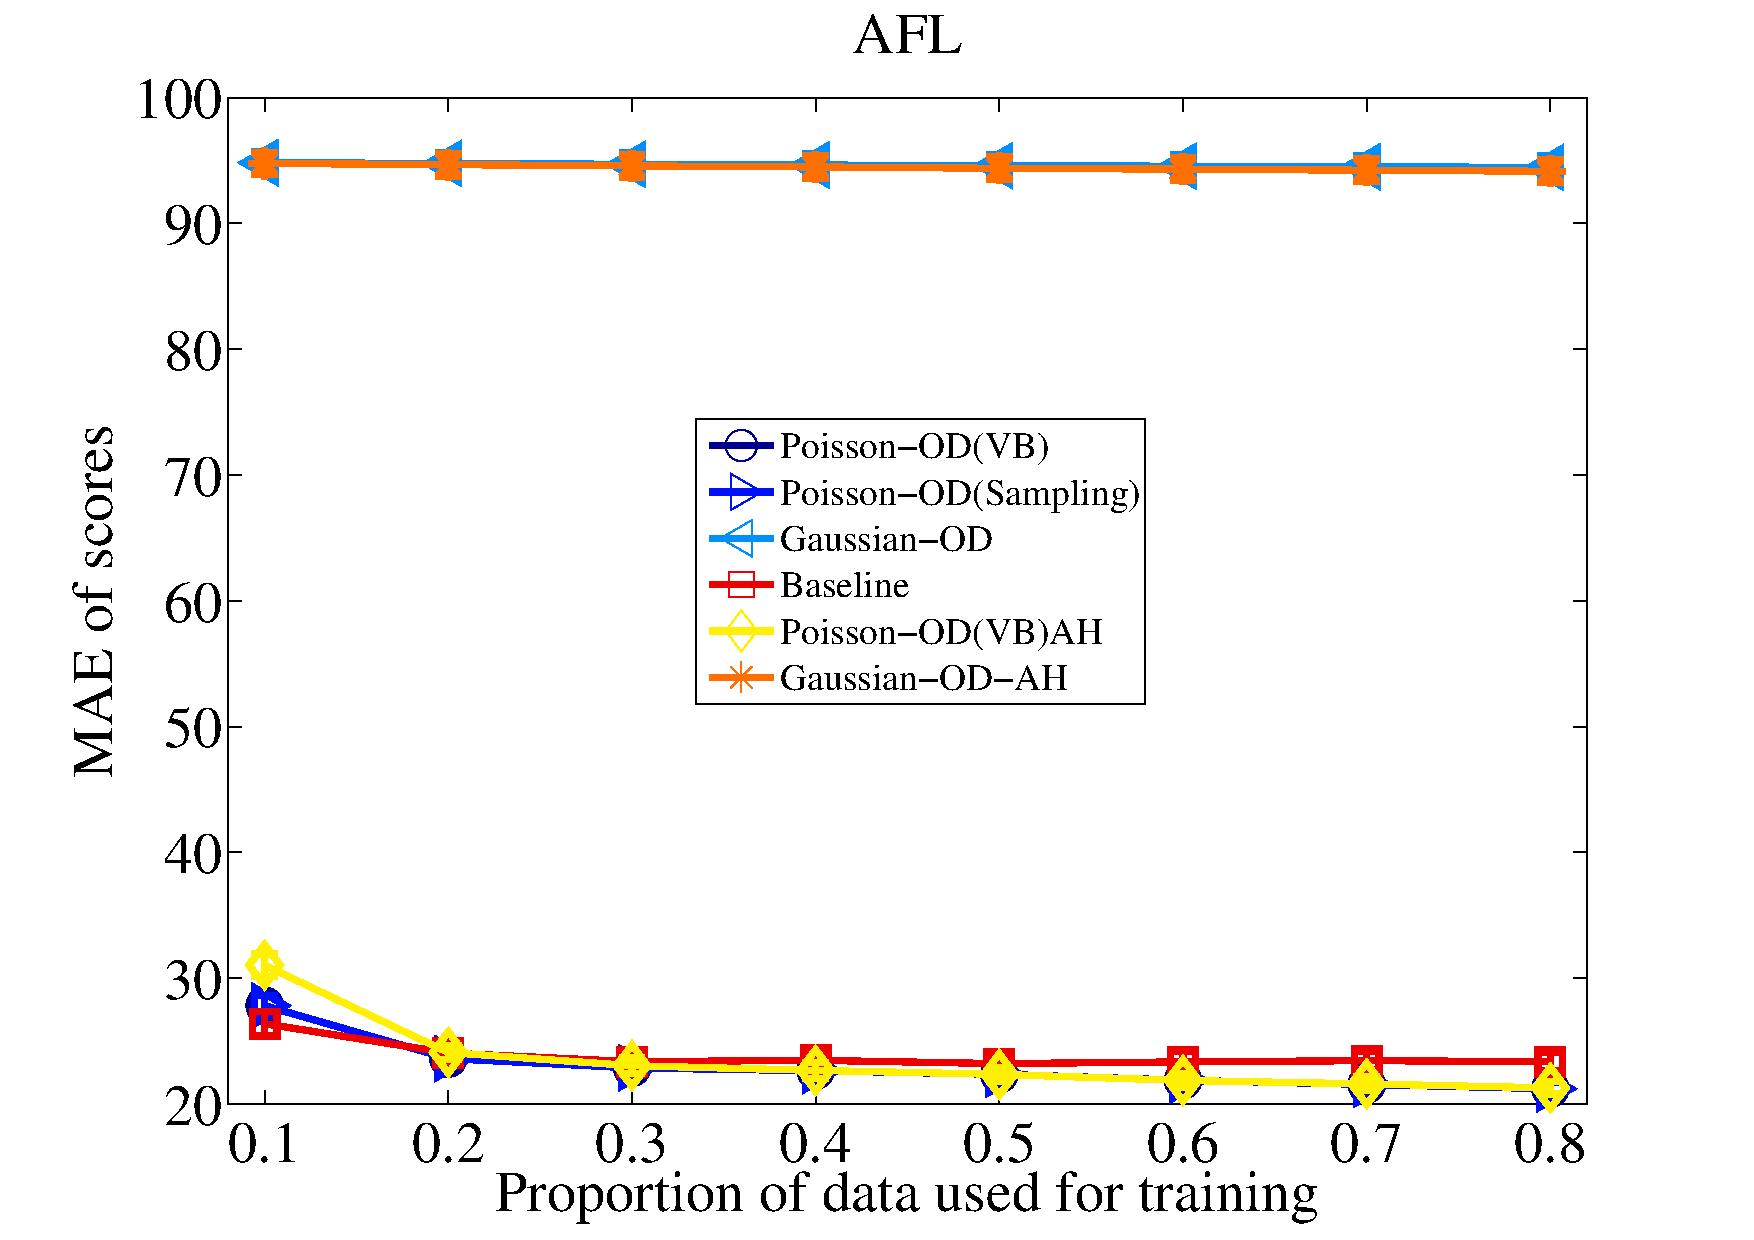
\epsfig{file=ScoreError_AFL, angle=0, height=7cm} 
}\\
\caption{\small Results on the UK-PL (upper), Halo (middle), and AFL (bottom), evaluated
using the Brier Score. Error bars indicate
95\% confidence intervals.}
\label{fig:ScoreError}
\end{figure}
\end{center}

\subsection{Variational Inference Vs. Sampling for the Poisson-OD Model}
\label{sec:VBSampling}
For the proposed Poisson-OD model, we studied the performance and efficiency for Bayesian inference based on the proposed variational Bayes, against one sampling method named slice sampling. For both the UK-PL and AFL data sets, we show the performance of the slice sampling for all evaluation criteria (see the Top and Bottom Panels of Figure~\ref{fig:InforGain}~\ref{fig:accuracyWLD}~\ref{fig:logLik}~\ref{fig:ScoreError}). We observed that the sampling approach only slightly performed better than the variational Bayes for a few training settings for the UK-PL data set, but the differences were not significant; for  most of the cases, these two approaches achieved comparable performances. 

Despite the similar performance between the variational Bayes and the slice sampling method for the Poisson-OD model, the slice sampling method required much longer time to obtain stationary samples for computing the statistics. Our empirical experiments indicated that the slice sampling took about 10 seconds when performing belief updating for an observation; however, the proposed fixed-point solution for the variational Bayes often converged after two or three iterations, which can be finished within less than 0.01 seconds, leading to 1000 times gain in computational efficiency. The gain in speed is extremely important for conducting online Bayesian skill learning for real-world matchmaking systems. Note that all the experiments were conducted on a laptop with an Intel i5 CPU, 4G memory, and codes are implemented in Matlab. Due to the high computational requirements for the sampling method, we omit the report of its performance for other data sets. Note that one can perhaps explore the advanced sampling approaches such as~\cite{Murray:AISTATS2010} to improve computational efficiency for the sampling method. 

\subsection{Model Home Field Improving Performance}
Home team advantages for many games particularly the football games has been encoded in different ways to improve match outcome prediction accuracy. To validate this known fact, we took the UK and AFL data sets where there is the notion of home field advantages. For the UK data set, we computed the probability that the home teams win the away teams in the following way. For each of the 41 teams of the UK data set, we first computed their win probability when playing on home fields, took the average win probability, and obtained its mean being 0.5665 with the standard deviation is 0.1511. Given this probability marginally larger than 0.5 with the large standard deviation, it is not clear if the home advantage can indeed help to predict WLD based match outcomes. This is reflected in the empirical evaluations for the four criteria reported in the previous sections, where we observed that the models with the home field advantages performed better for limited cases. 

For the AFL data set, we conducted the same analysis, and obtained an average win probability across the 16 teams being 0.5907 (with the standard deviation being 0.1381), larger than that for the UK data set. Referring back to our empirical evaluations for the AFL data set in the bottom panels of Figure~\ref{fig:InforGain}~\ref{fig:accuracyWLD}~\ref{fig:logLik}, we indeed observed that the modeling of home field advantages led to the slightly better performance, particularly for the Poisson-OD model. 